\documentclass[12pt,a4paper]{report}

% --- Paquetes de Idioma y Codificación ---
\usepackage[utf8]{inputenc}
\usepackage[T1]{fontenc}
\usepackage[spanish, es-tabla]{babel}

% --- Diseño de Página ---
\usepackage{geometry}
\geometry{top=2.5cm, bottom=2.5cm, left=3cm, right=3cm}

% --- Matemáticas y Símbolos ---
\usepackage{amsmath, amssymb, amsthm}

% --- Colores y Cajas ---
\usepackage[dvipsnames]{xcolor}
\usepackage[most]{tcolorbox}

% Caption

\usepackage{caption}

% Gráficos

\usepackage{graphicx}

% Espaciadora

\newcommand{\esp}{\vspace{0.5cm}}

% promedio

\newcommand{\prom}[1]{\left\langle #1 \right\rangle}

% ket

\newcommand{\ket}[1]{| #1 \rangle}

% bra

\newcommand{\bra}[1]{\langle #1 |}

% braket

\newcommand{\braket}[2]{\langle #1 | #2 \rangle}

% Bibliografía

\usepackage[style=apa, backend=biber]{biblatex} % Estilo APA
\addbibresource{biblio.bib} % Nombre de tu archivo .bib

% Configuración de cajas personalizadas
\newtcolorbox{importante}{
	colback=red!5!white,
	colframe=red!75!black,
	title=Importante,
	fonttitle=\bfseries
}

\newtcolorbox{nota}{
	colback=blue!5!white,
	colframe=blue!75!black,
	title=Nota,
	fonttitle=\bfseries
}

% Definición de la caja de bibliografía
\newtcolorbox{bibliografia}{
	colback=gray!5!white,
	colframe=gray!75!black,
	title=Bibliografías útiles,
	fonttitle=\bfseries,
	breakable
}

% Socrative para óptica 2

\newtcolorbox{Socrative}{
	colback=orange!5!white,
	colframe=orange!75!black,
	title=Socrative,
	fonttitle=\bfseries,
	breakable
}

% Float

\usepackage{float}

% --- Hipervínculos ---
\usepackage{hyperref}
\hypersetup{
	colorlinks=true,
	linkcolor=blue,
	filecolor=magenta,      
	urlcolor=cyan,
}

% --- Datos del Documento ---
\title{Statistical Physics}
\author{Chengyu Jin}
\date{\today}

\begin{document}
	
	\maketitle
	
	\tableofcontents
	\newpage
	
	\chapter{Microcanonical Ensemble}
	
	\section{Introduction}
	
	\begin{figure}[H]
		\centering
		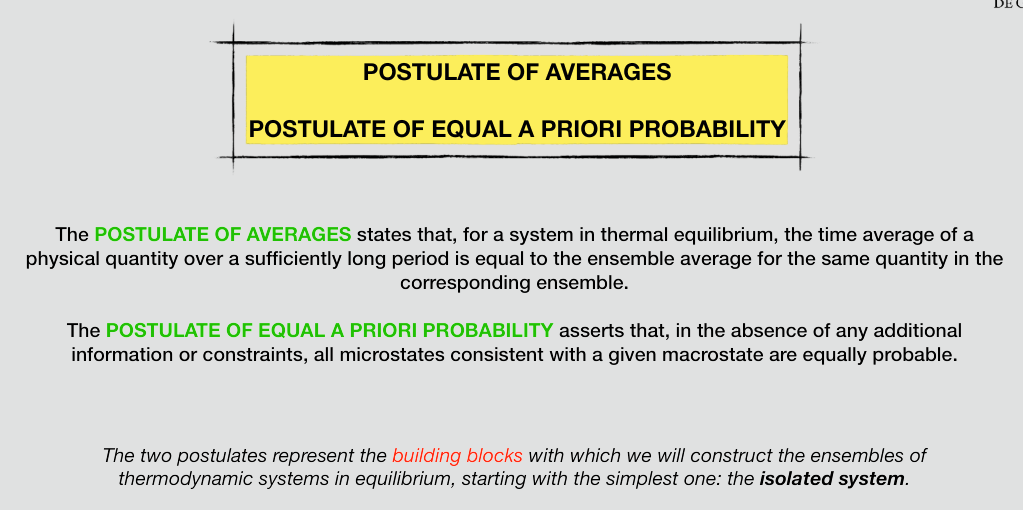
\includegraphics[width=0.7\textwidth]{IMG/int.png}
	\end{figure}
	
	\esp
	
	We have stressed in the \textit{Introduction} that a macroscopic system consists of approximately $N = 10^{23}$ particles and, correspondingly, exhibits an energy spectrum that varies within $\Delta E \sim e^{-N}$. Any attempt to find a solution of the equations of motion at the microscopic level is hopeless and also superfluous as during the measurement process (which takes a finite amount of time) both macroscopic and microscopic properties of the system change. We have also learnt that a many-body system cannot be characterised by a single microstate, but rather by an \textbf{ensemble of microstates} which is determined by macroscopic variables ($E, V, N, \dots$). Experience shows that, at sufficiently long time scales, any microscopic system evolves towards an equilibrium state, in which
	
	\esp
	
	\begin{equation}
		\frac{\partial \hat{\rho}}{\partial t} = -\frac{i}{\hbar} [\hat{H}, \hat{\rho}] = 0
		\label{eq:von}
	\end{equation}
	
	\esp
	
	\begin{figure}[H]
		\centering
		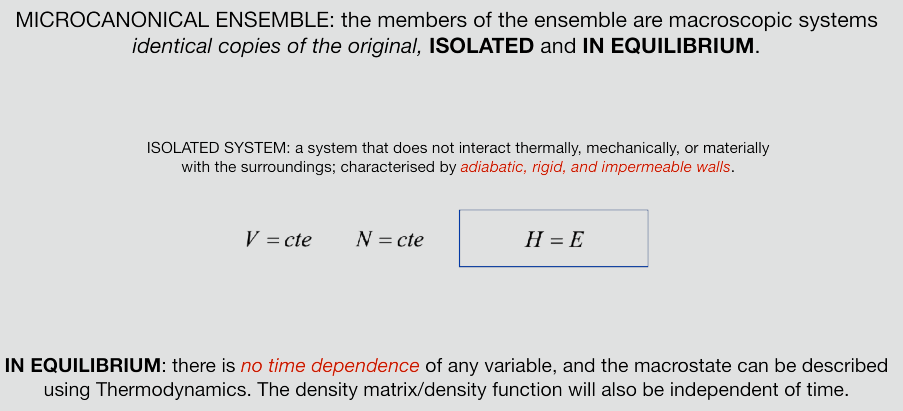
\includegraphics[width=0.7\textwidth]{IMG/int2.png}
	\end{figure}
	
	\esp
	
	must be satisfied. Since, according to Eq. (\ref{eq:von}), the density operator commuted with the Hamiltonian operator, in an equilibrium ensemble $\rho$ can depend only on conserved quantities, the microscopic properties of the system change continually even at equilibrium, but the distribution of microstates within the ensemble does not depend on time. In this chapter, to fix these ideas, we will introduce the microcanonical ensemble, where number of particles ($N$), system volume ($V$) and energy ($E$) are constant. To this end, we will make use of the \textit{Postulate of Averages} and \textit{Postulate of Equal A Priori Probability}. These postulates are the building blocks with which we will construct the thermodynamic ensembles in equilibrium, starting with the simplest: the isolated system.
	
	\esp
	
	\begin{figure}[H]
		\centering
		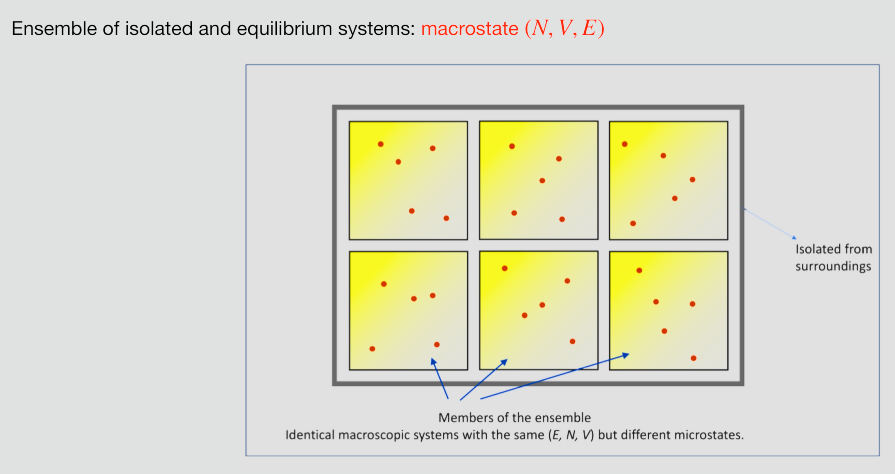
\includegraphics[width=0.7\textwidth]{IMG/censemble.png}
	\end{figure}
	
	\esp
	
	The members of the microcanonical ensemble are macroscopic systems identical to the original, \textbf{isolated}, and \textbf{in equilibrium}. An isolated system does not interact thermally, mechanically, or materially with the outside; it has adiabatic, rigid, and impermeable walls. As such, it exhibits constant volume, constant number of particles. Additionally $H = E$. Systems in equilibrium have no temporal dependencies on any variable, and their macrostate can be described using thermodynamics. The density matrix/function also does not depend on time.
	
	\section{Classical Microcanonical Ensemble}

	\begin{figure}[H]
		\centering
		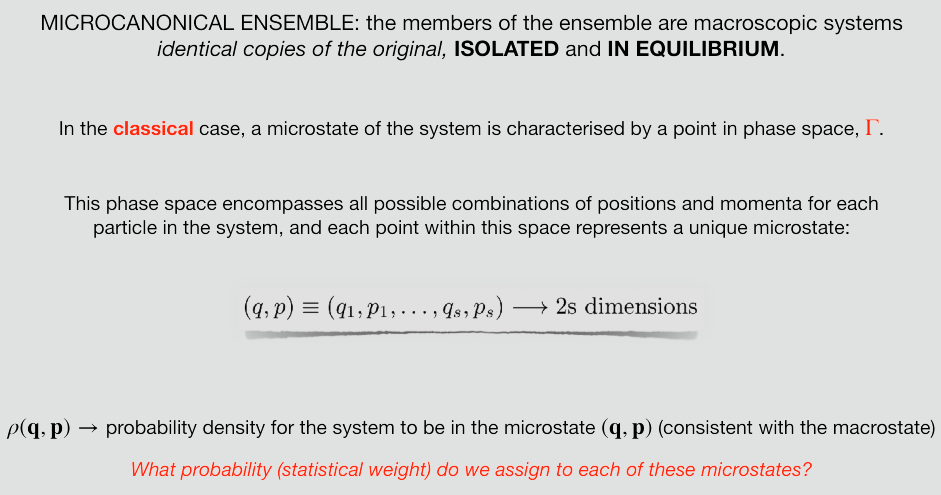
\includegraphics[width=0.7\textwidth]{IMG/censemble2.png}
	\end{figure}
	
	\esp
	
	In the microcanonical ensemble, the constituents of the ensemble represent macroscopic systems that are exact copies of the original system. These systems are kept in isolation, do not interact with the external environment, and are maintained in a state of thermodynamic equilibrium. In the classical context, a microstate of the system is distinctly characterised by a specific point within the system's phase space, denoted as $\Gamma$. This phase space \textbf{encompasses all possible combinations of positions and momenta for each particle in the system, and each point within this space represents a unique microstate}:
	
	\esp
	
	\begin{equation}
		(\mathbf{q}, \mathbf{p}) \equiv (q_1, p_1, \dots, q_s, p_s) \longrightarrow 2s \text{ dimensions}
	\end{equation}
	
	\esp
	
	The probability density associated with the likelihood of the system being in a given microstate, $\rho(q, p)$, characterises the relative probability of finding the system in that specific microstate defined by its generalised coordinates $q$ and momenta $p$ within the phase space. In a sense, it quantifies the ''crowding'' of microstates within the phase space, indicating which microstates are more or less probable within the constraints of the given macrostate.
	
	\esp
	
	\begin{figure}[H]
		\centering
		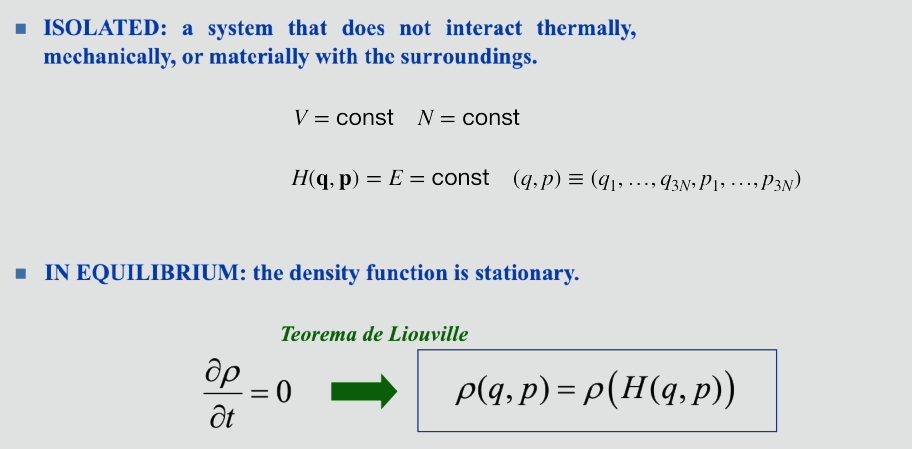
\includegraphics[width=0.7\textwidth]{IMG/censemble3.png}
	\end{figure}
	
	\esp
	
	What probability (statistical weight) do we assign to each of these microstates? We know that our system is isolated and in equilibrium. This implies that $N, V$ and $E$ are constant and the density function does not change with time. Now, what is the density function for the microcanonical ensemble? 
	
	\begin{figure}[H]
		\centering
		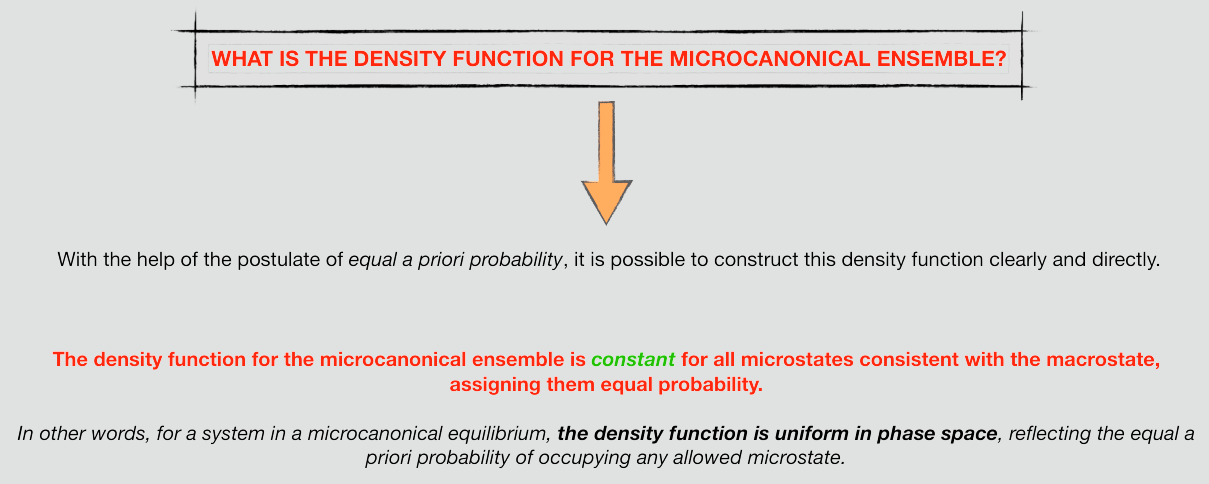
\includegraphics[width=0.7\textwidth]{IMG/censemble4.png}
	\end{figure}
	
	With the help of the postulate of equal a priori probability, it is possible to construct this density function clearly and directly. In the microcanonical ensemble, all microstates compatible with a particular macrostate have the same probability of occurring, simplifying the construction of the density function. Generally speaking:
	
	\esp
	
	\begin{equation}
		\rho(\mathbf{q}, \mathbf{p}) = \begin{cases} \text{constant} & \text{if } (\mathbf{q}, \mathbf{p}) \text{ is compatible with the macrostate} \\ 0 & \text{otherwise} \end{cases}
	\end{equation}
	
	\esp
	
	\noindent The constant in this function is chosen in such a way that the \textbf{sum or integral of the density function over the entire phase space $(q, p)$ equals 1}, ensuring that the total probability of finding the system in some microstate within the macrostate is 1. Let's now add some specific details:
	
	
	\begin{enumerate}
		\item In any average within this ensemble, it must be taken into account that all mechanical states $(q, p)$ for which $H \neq E$ cannot contribute to the mean value, as they do not conserve energy (see Fig. 4.4).
		\item $\rho$ is exclusively a function of $H$.
		\item Equal a priori probability for all microstates with $H = E$.
		\item Normalization condition:
		
		\esp
		
		\begin{equation}
			\int \rho(\mathbf{q}, \mathbf{p}) \, d\mathbf{q} \, d\mathbf{p} = 1.
		\end{equation}
	\end{enumerate}
	
	\esp
	
	\subsection{Density of States}
	
	\begin{figure}[H]
		\centering
		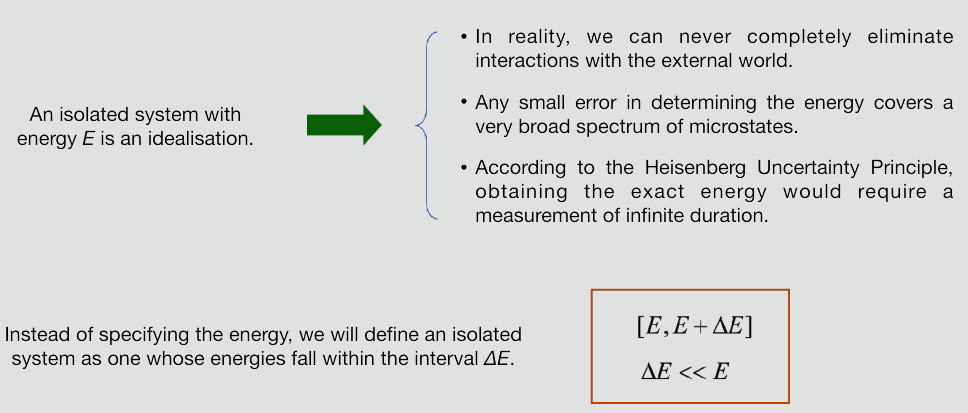
\includegraphics[width=0.7\textwidth]{IMG/censemble5.png}
	\end{figure}
	
	\esp
	
	An isolated system with a precisely defined energy $E$ is an idealisation. In reality, we can never completely eliminate interactions with the external world. Any small error in determining the energy covers an extremely wide spectrum of microstates. According to the \textit{Heisenberg Uncertainty Principle}, obtaining the energy exactly would require a measurement of infinite duration. As such, instead of specifying the energy precisely, we define an isolated system as one whose energies fall within the interval $[E, E + \Delta E]$ with $\Delta E \ll E$. 
	
	\esp
	
	\begin{figure}[H]
		\centering
		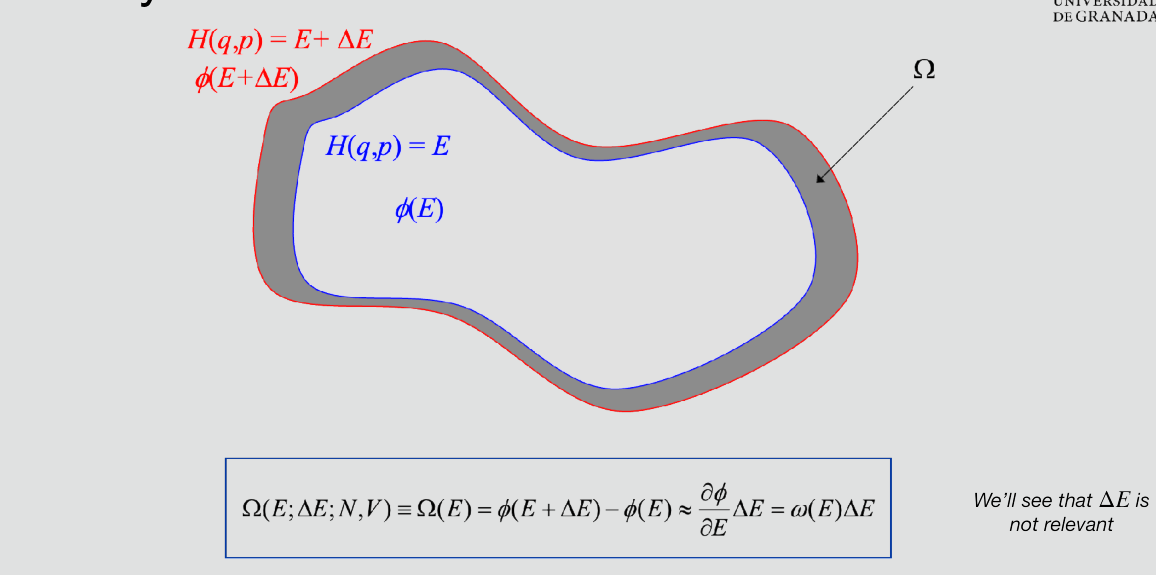
\includegraphics[width=0.7\textwidth]{IMG/density.png}
	\end{figure}
	
	\esp
	
	In particular, we consider a small but finite shell $[E, E + \Delta E]$ close to the energy surface. With reference to Fig. 4.3, $\Omega(N, V, E)$ is the volume of the shell bounded by the two energy surfaces with energies $E$ and $E + \Delta E$ or, equivalently, the volume of phase space accessible to a system with $N$ particles, volume $V$, and total energy $E$. In other words, $\Omega(N, V, E)$ quantifies the number of microstates available to the system under those conditions:
	
	\esp
	
	\begin{equation}
		\Omega(N, V, E) = \int_{E \leq H \leq E + \Delta E} d\mathbf{q} \, d\mathbf{p}
	\end{equation}
	
	\esp
	
	\noindent Let now $\phi$ be the total volume of phase space enclosed by the energy surface $E$. We then have that
	
	\esp
	
	\begin{equation}
		\Omega(N, V, E) = \phi(E + \Delta E) - \phi(E)
	\end{equation}
	
	\esp
	
	\noindent Taking the limit for $\Delta E \to 0$, corresponding to an infinitesimal shell, one obtains
	
	\esp
	
	\begin{equation}
		\Omega(N, V, E) \approx \frac{\partial \phi(E)}{\partial E} \Delta E \equiv \omega \Delta E, \quad \Delta E \ll E
	\end{equation}
	
	\esp
	
	$\Omega(N, V, E)$ refers to the \textit{microcanonical ensemble multiplicity}. It represents the number of microstates that correspond to a specific energy $E$ in a microcanonical ensemble. In other words, $\Omega(N, V, E)$ quantifies the \textbf{number of distinct ways in which the energy $E$ can be distributed among the particles in the system} while satisfying the fixed constraints of $N$ and $V$. 
	
	\esp
	
	\begin{figure}[H]
		\centering
		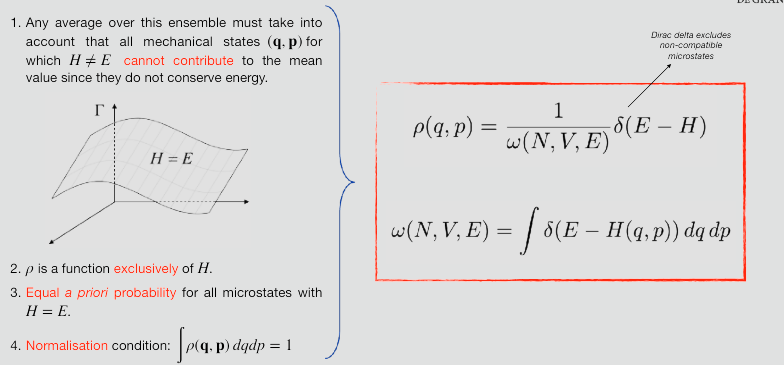
\includegraphics[width=0.7\textwidth]{IMG/density2.png}
	\end{figure}
	
	\esp
	
	From $\Omega$ and its dependence on the variables $N, V$, and $E$, the entire thermodynamics of the microcanonical ensemble can be deduced. Additionally, the normalisation constant
	
	\esp
	
	\begin{equation}
		\omega(N, V, E) = \frac{\partial \phi(E)}{\partial E} = \int \delta(E - H(\mathbf{q}, \mathbf{p})) d\mathbf{q} \, d\mathbf{p}
	\end{equation}
	
	\esp
	
	represents the \textbf{density of states}, indicating the number of compatible microstates per unit energy interval. By contrast, $\Omega$ gives the total volume of phase space accessible to the system, quantifying the number of microstates available under specified conditions.
	
	\esp
	
	Let's see how the density of states is related to the phase-space density $\rho(\mathbf{q}, \mathbf{p})$, which describes how microstates are distributed in phase space (remember this is a probability!). In the microcanonical ensemble, all accessible states are equally probable, meaning:
	
	\esp
	
	\begin{equation}
		\rho(\mathbf{q}, \mathbf{p}) \propto \delta(H(\mathbf{q}, \mathbf{p}) - E)
	\end{equation}
	
	\esp
	
	\noindent Since the system is equally likely to be in any of these microstates, the normalisation factor must ensure that:
	
	\esp
	
	\begin{equation}
		\int \rho(\mathbf{q}, \mathbf{p}) \, d\mathbf{q} \, d\mathbf{p} = 1
	\end{equation}
	
	\esp
	
	\noindent Using the definition of $\omega(E)$, we then set:
	
	\esp
	
	\begin{equation}
		\rho(\mathbf{q}, \mathbf{p}) = \frac{\delta(H(\mathbf{q}, \mathbf{p}) - E)}{\omega(E)}
	\end{equation}
	
	\esp
	
	\noindent where the Dirac delta excludes non-compatible microstates. Equivalently,
	
	\esp
	
	\begin{equation}
		\rho(\mathbf{q}, \mathbf{p}) = \begin{cases} \frac{1}{\omega(E)} & E \leq H(\mathbf{q}, \mathbf{p}) \leq E + \Delta E \\ 0 & \text{otherwise} \end{cases}
	\end{equation}
	
	\esp
	
	\begin{figure}[H]
		\centering
		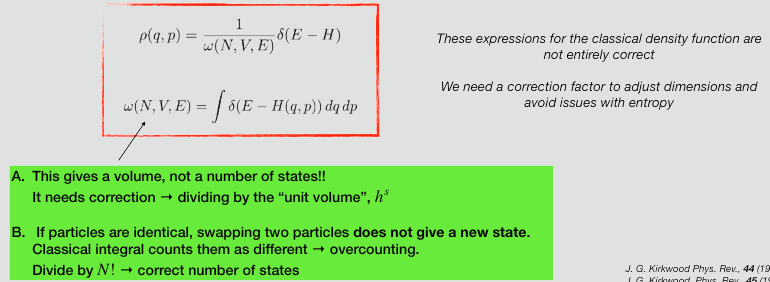
\includegraphics[width=0.7\textwidth]{IMG/density3.png}
	\end{figure}
	
	\esp
	
	The expressions given above for the classical density function provide a useful framework for understanding the statistical behaviour of macroscopic systems in the classical realm. However, it's important to note that these classical expressions may not hold true when we transition to the quantum realm. The behaviour of particles at the quantum level is inherently probabilistic and governed by the Heisenberg uncertainty principle, which is encapsulated in $h$. Boltzmann realised that the particles in the system are actually indistinguishable. This implies dividing the number of states $\omega(E)$ by an additional $N!$, thereby accounting for the number of different ways to label the particles. Additionally, to satisfy dimensional requirements, Boltzmann suggested to use a constant that has units of momentum times length, which we now know to be $h^s$, with $h$ the Planck constant and $s$ the number of degrees of freedom of the system. The interested reader is referred to McQuarrie, p. 114 for further details [3]. In particular,
	
	\esp
	
	\begin{equation}
		\Delta q_i \Delta p_i \sim h
	\end{equation}
	
	\esp
	
	\begin{equation}
		\Delta q^{(s)} \Delta p^{(s)} \sim h^{(s)}
	\end{equation}

	\esp
	
	\begin{figure}[H]
		\centering
		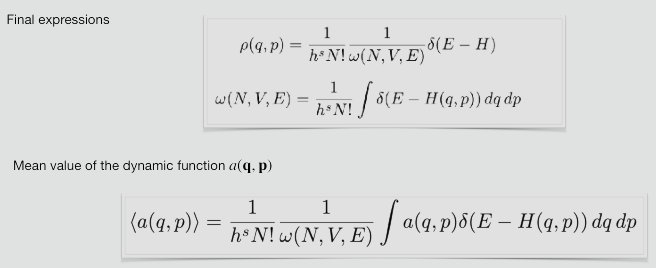
\includegraphics[width=0.7\textwidth]{IMG/density4.png}
	\end{figure}
	
	\esp
	
	\noindent We therefore end up with the following final expressions:
	
	\esp
	
	\begin{equation}
		\rho(\mathbf{q}, \mathbf{p}) = \frac{1}{h^s N!} \frac{1}{\omega(N, V, E)} \delta(E - H)
	\end{equation}
	
	\esp
	
	\begin{equation}
		\omega(N, V, E) = \frac{1}{h^s N!} \int \delta(E - H(\mathbf{q}, \mathbf{p})) \, d\mathbf{q} \, d\mathbf{p}
	\end{equation}
	
	\esp
	
	\noindent The mean value of the dynamic function is given by:
	
	\esp
	
	\begin{equation}
		\langle a(\mathbf{q}, \mathbf{p}) \rangle = \frac{1}{h^s N!} \frac{1}{\omega(N, V, E)} \int a(\mathbf{q}, \mathbf{p}) \delta(E - H(\mathbf{q}, \mathbf{p})) \, d\mathbf{q} \, d\mathbf{p}
	\end{equation}
	
	\esp
	
	\noindent and the number of states with energy in the interval $[0, E]$ reads
	
	\esp
	
	\begin{equation}
		\phi(N, V, E) \equiv \phi(E) = \frac{1}{h^s N!} \int \theta(E - H) \, d\mathbf{q} \, d\mathbf{p}, \quad \text{with } \theta(x) = \begin{cases} 1 & \text{if } x > 0 \\ 0 & \text{if } x < 0 \end{cases}
	\end{equation}
	
	\esp
	
	\noindent where $\theta$ is the Heaviside step function.
	
	\esp
	
	\begin{figure}[H]
		\centering
		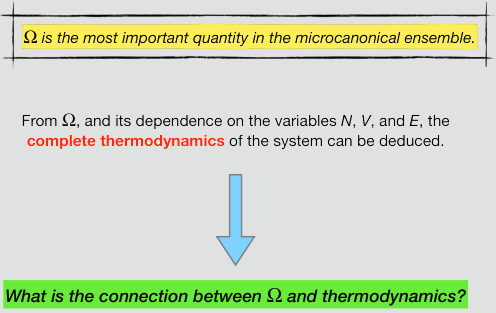
\includegraphics[width=0.7\textwidth]{IMG/density5.png}
	\end{figure}

	\printbibliography[title={Bibliografía}]
\end{document}